% Copyright 2004 by Till Tantau <tantau@users.sourceforge.net>.
%
% In principle, this file can be redistributed and/or modified under
% the terms of the GNU Public License, version 2.
%
% However, this file is supposed to be a template to be modified
% for your own needs. For this reason, if you use this file as a
% template and not specifically distribute it as part of a another
% package/program, I grant the extra permission to freely copy and
% modify this file as you see fit and even to delete this copyright
% notice. 

\documentclass{beamer}
%\documentclass[12pt]{article}
%\usepackage[noxcolor]{beamerarticle}

\usepackage{graphicx}
\usepackage{hyperref}
\usepackage{amssymb}
\usepackage{amsthm}
\usepackage{amsmath}
\usepackage{tikz,tikz-qtree}
\usepackage{caption}
\usepackage{subcaption}
\usepackage{biblatex}
\usepackage{threeparttablex,booktabs}
\usepackage{makecell}
\usepackage{bm}
\usepackage{xcolor}

\definecolor{OliveGreen}{rgb}{0,0.6,0}

% There are many different themes available for Beamer. A comprehensive
% list with examples is given here:
% http://deic.uab.es/~iblanes/beamer_gallery/index_by_theme.html
% You can uncomment the themes below if you would like to use a different
% one:
%\usetheme{AnnArbor}
%\usetheme{Antibes}
%\usetheme{Bergen}
%\usetheme{Berkeley}
%\usetheme{Berlin}
%\usetheme{Boadilla}
%\usetheme{boxes}
\usetheme{CambridgeUS}
%\usetheme{Copenhagen}
%\usetheme{Darmstadt}
%\usetheme{default}
%\usetheme{Frankfurt}
%\usetheme{Goettingen}
%\usetheme{Hannover}
%\usetheme{Ilmenau}
%\usetheme{JuanLesPins}
%\usetheme{Luebeck}
%\usetheme{Madrid}
%\usetheme{Malmoe}
%\usetheme{Marburg}
%\usetheme{Montpellier}
%\usetheme{PaloAlto}
%\usetheme{Pittsburgh}
%\usetheme{Rochester}
%\usetheme{Singapore}
%\usetheme{Szeged}
%\usetheme{Warsaw}


% reset footnote size in beamer
\setbeamerfont{footnote}{size=\tiny}
\captionsetup{width=10cm}

\title{Financial Reform and Liberalization in China}

% A subtitle is optional and this may be deleted
% \subtitle{MODELLING THE POTENTIAL IMPACT OF FINANCIAL \\
% REFORM AND LIBERALIZING IN CHINA}

\author{
    Zeming Wang\inst{1} \and 
    Supervisor: Paul Gretton\inst{2}
    }
% - Give the names in the same order as the appear in the paper.
% - Use the \inst{?} command only if the authors have different
%   affiliation.

\institute[] % (optional, but mostly needed)
{
  \inst{1}%
  College of Business and Economics
  \and
  \inst{2}%
  East Asian Bureau of Economic Research
}
% - Use the \inst command only if there are several affiliations.
% - Keep it simple, no one is interested in your street address.

\date{Nov. 2017}
% - Either use conference name or its abbreviation.
% - Not really informative to the audience, more for people (including
%   yourself) who are reading the slides online

\subject{Economics}
% This is only inserted into the PDF information catalog. Can be left
% out. 

% If you have a file called "university-logo-filename.xxx", where xxx
% is a graphic format that can be processed by latex or pdflatex,
% resp., then you can add a logo as follows:

% \pgfdeclareimage[height=0.5cm]{university-logo}{university-logo-filename}
% \logo{\pgfuseimage{university-logo}}

% Delete this, if you do not want the table of contents to pop up at
% the beginning of each subsection:
% \AtBeginSubsection[]
% {
%   \begin{frame}<beamer>{Outline}
%     \tableofcontents[currentsection,currentsubsection]
%   \end{frame}
% }

\addbibresource{ref.bib}%

% Let's get started
\begin{document}

\begin{frame}
  \titlepage
\end{frame}

% \begin{frame}{Outline}
%   \tableofcontents
%   % You might wish to add the option [pausesections]
% \end{frame}

% Section and subsections will appear in the presentation overview
% and table of contents.
\section{Motivation}
\subsection{Research Questions}

\begin{frame}{Motivation}
\begin{itemize}
\item China's financial reform lagging behind real sector reforms
\item What's the consequence of financial repressive policies?
\item What's the potential benefit of financial liberalization?
\item What's the potential risk of such financial reforms?
\end{itemize}
\end{frame}

\section{Finance and Growth}
\subsection{Theories}
\begin{frame}{Financial Development and Economic Growth}
\begin{itemize}
\item Reduce transaction cost
\item Reduce information cost
\item Mobilize savings
\item Allocate resources
\item Facilitate liquidity
\item Ameliorate risk
\item Exert corporate control
\end{itemize}
\end{frame}

\subsection{Repressive Policies}
\begin{frame}{Financial Restrictive Policies}
\begin{itemize}
\item State-owned banks and enterprises
\item Interest-rate controls
\item Financial institution licensing
\item Government designating investment
\item Approval-based IPO system
\item Capital account quota
\end{itemize}    
\end{frame}

\section{Financial Repression in China}
\subsection{Overall Index}
\begin{frame}{Financial Repression in China}{Financial Development Index}
\begin{figure}
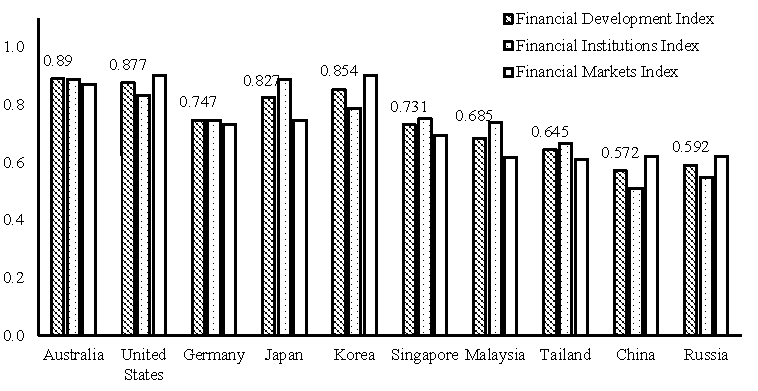
\includegraphics[scale=.75]{fig/findev.pdf}
\end{figure}
\tiny
\emph{Note: }
The index is constructed using 33 years of annual data between 1980 and 2013 for
183 countries worldwide by measuring three dimensions -- depth, access and 
efficiency -- of both financial institutions and financial markets.\\
\emph{Source}: 
Based on Svirydzenka, 2016 (IMF)\footfullcite{sviry2016}.
\end{frame}

\subsection{Interest Rate Fragmentation}

\begin{frame}{State-Owned Banking System}{Interest Rate Fragmentation}
\begin{figure}
\centering
\begin{subfigure}{.5\textwidth}
  \centering
  \includegraphics[scale=.45]{fig/lrate.pdf}
  \caption{\footnotesize{Various Lending Rate}}
\end{subfigure}%
\begin{subfigure}{.5\textwidth}
  \centering
  \includegraphics[scale=.4]{fig/realr.pdf}
  \caption{\footnotesize{Real Interest Rate}}
\end{subfigure}
\end{figure}
\tiny
\emph{Note: } 
Wenzhou private lending rate is based on the Wenzhou composite lending rate index,
which is the private lending rate in Wenzhou and is published officially by the 
government of Wenzhou. 
P2P network lending rate is the average lending rate of online P2P platforms. 
Before 2015, China's central bank directly controls commercial banks' interest rate.
After 2015, commercial banks can freely float their interest rate, though the 
central bank still sets a reference rate.\\
\emph{Source: } 
CEIC, World Bank.
\end{frame}

\subsection{Inefficient Resource Allocation}
\begin{frame}{Inefficient Resource Allocation}{Imbalanced Sector Development}
\begin{figure}
\centering
\includegraphics[scale=.75]{fig/roa-cn.pdf}
\end{figure}
\tiny
\emph{Note:} 
The values reported here are calculated from the data of the companies listed 
on the stock market. The number of companies consisted in each sector are 
also meaningful, and are thus reported here: energy (84), materials (537), 
industries (810), consumer discretionary (534), consumer staples (211), 
health care (226), finance and real estate (224), technology (464), 
telecom (94), and utilities (96).\\
\emph{Source}:
Based on data from \textit{lixinger.com}.
\end{frame}

\subsection{Capital Deepening}
\begin{frame}{Capital Deepening}{Still Low Capital Intensity}
\begin{figure}
\centering
\begin{subfigure}{.5\textwidth}
\centering
\includegraphics[scale=.45]{fig/invest.pdf}
\caption{Gross capital formation (\% of GDP)}
\label{fig:invest}
\end{subfigure}%
\begin{subfigure}{.5\textwidth}
\centering
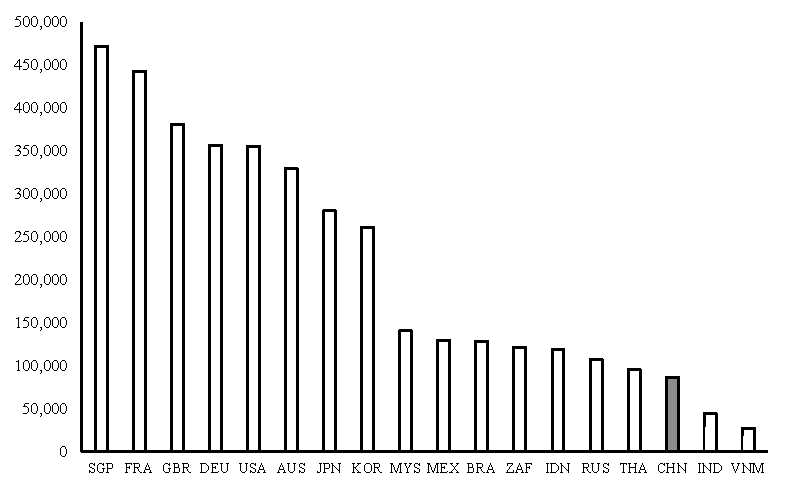
\includegraphics[scale=.45]{fig/capital-pc.pdf}
\caption{Capital stock per worker (2014)}
\label{fig:capital-pc}
\end{subfigure}
%\caption{Investment and Capital per Worker}
\tiny\raggedright 
\emph{Note:} 
Capital values are converted using purchasing power parity, and shown in 2011 US\$. \\
\emph{Source:}
The World Bank, Penn World Table Version 8.0.
\end{figure}    
\end{frame}


% \subsection{Prohibitive Policies}
% \begin{frame}{Financial Policies and Economic Growth}{Productive or Prohibitive?}
% \begin{figure}
% \centering
% \includegraphics[scale=.55]{fig/frep.pdf}
% \end{figure}
% \tiny
% \emph{Note:} 
% This figure shows the coefficients estimated by Huang and Wang (2011) of the 
% effects of each repressive policy on economic growth. These repressive policies are 
% state-owned banks in total bank loans (SOB), the share of the state sector in 
% total outstanding loans (PCR), reserve requirement ratio (SRR), interest rate 
% control (ICI), real deposit rate (RID) and capital account control (CAC).
% FREP is the overall financial repression index that constructed from the above 
% six variables. \\
% \emph{Source:}
% Based on estimations by Huang and Wang (2011)\footfullcite{huang2011}.
% \end{frame}


\section{Simulation}
\subsection{GTAP Overview}
\begin{frame}{Financial Reform}{Modelling with GTAP}
\begin{itemize}
\item<1-> Need for financial reform is consensus among Chinese leaders 
\item<2-> What is the potential benefit of financial liberalization?
\item<3-> Simulation with GTAP (Global Trade Analysis Project) 
    \begin{itemize}
    \item General equilibrium model
    \item Open economy with fixed exchange rate
    \item Labor mobility across industries, but not across countries
    \end{itemize}
\item<4-> How to model financial reform in GTAP?
\end{itemize}   
\end{frame}

\subsection{An increase in productivity of financial services}
\begin{frame}{Simulation I}{An increase in productivity of financial services}
\begin{itemize}
\item<1-> Financial Service Provider
$$ Y = F(X_1, X_2, \dots, X_n) $$
\item<2-> Increase in productivity of financial service 
$$ Y = \underset{\uparrow}{\bm{A}} 
   F(X_1,X_2, \dots, X_n)
$$
\item<3-> In GTAP's language:
\begin{center}
\textbf{Shock} \textcolor{OliveGreen}{avaall}
(``\textit{\textcolor{red}{FinBus}}", ``CHN") =
\textbf{uniform} 1.0 \\
\textbf{Shock} \textcolor{OliveGreen}{afall}
(..., ``\textit{\textcolor{red}{FinBus}}", ``CHN") = 
\textbf{uniform} 1.0 \\
\end{center}
\end{itemize}
\end{frame}

\begin{frame}{Simulation Result I}{An increase in productivity of financial services}
\begin{table}
\begin{threeparttable}
% \caption{Simulation Result of an Increase in 
% Productivity of Finance Service in China}
% \label{tab:sim-pfin}
\def\theadset{\def\arraytretch{1.5}}
\def\arraystretch{1.2}
\small
\begin{tabular}{lcccc}
\hline\hline
    & \thead{Read GDP\\\emph{\% change}} 
    & \thead{Capital accumulation\\\emph{\% change}} 
    & \thead{Trade balance to\\income ratio} \\
\hline
CHN & 4.392 &	11.130 & 0.018 \\
AUS & 0.132 &	0.256 & -0.003 \\
USA & 0.022 &	0.053 & -0.002 \\
EU  & 0.000 &	0.015 & -0.002 \\
ROW & 0.033 &	0.041 & -0.002 \\
\hline\hline
\end{tabular}
\begin{tablenotes}[para, flushleft]
\emph{Note:} Modelled as a uniform 1\% increase in value-added augmenting 
technology in the financial sector change, together with a uniform 1 point 
increase in financial intermediate input augmenting technology for other 
industries that take financial services as intermediate inputs.\\
% The model is solved using Gragg's method; the accuracy requirement is set 
% to that at least 99\% of the variables are accurate to at least 4 figures. 
% The extrapolation accuracy shows that we can be confident for 6 figure 
% accuracy for most variables.\\
\emph{Source:} Author estimated.
\end{tablenotes}
\end{threeparttable}
\end{table}
\end{frame}


\subsection{An increase in productivity of capital}
\begin{frame}{Simulation II}{An increase in productivity of capital}
\begin{itemize}
\item<1-> Firm's production function
$$ Y = F(K,L) $$
\item<2-> Increase in productivity of capital 
$$ Y = F(\underset{\uparrow}{\bm{\lambda}} K, L)
$$
\item<3-> In GTAP's language:
\begin{center}
\textbf{Shock} \textcolor{OliveGreen}{afeall}
(``\textit{\textcolor{red}{capital }}",..., ``CHN") =
\textbf{uniform} 1.0 
\end{center}
\end{itemize}
\end{frame}

\begin{frame}{Simulation Result II}{An increase of productivity of capital}
\begin{table}
\begin{threeparttable}
% \caption{Simulation Result of an Increase in 
% Productivity of Capital in China}
% \label{tab:sim-pcap}
\def\theadset{\def\arraytretch{1.5}}
\def\arraystretch{1.2}
\small
\begin{tabular}{lcccc}
\hline\hline
    & \thead{Read GDP\\\emph{\% change}} 
    & \thead{Capital accumulation\\\emph{\% change}} 
    & \thead{Trade balance to\\income ratio} \\
\hline
CHN & 4.807 &	11.624 & 0.018 \\
AUS & 0.142 &	0.279 & -0.003 \\
USA & 0.021 &	0.048 & -0.002 \\
EU  & -0.005 &	0.005 & -0.002 \\
ROW & 0.030 &	0.036 & -0.002 \\
\hline\hline
\end{tabular}
\begin{tablenotes}[para,flushleft]
\emph{Note:} Modelled as a uniform 1\% increase in primary augmenting 
technology for capital.
The model is solved using Gragg's method; the accuracy requirement is set 
to that at least 99\% of the variables are accurate to at least 4 figures. 
The extrapolation accuracy shows that we can be confident for 6 figure accuracy 
for most variables.\\
\emph{Source:} Author estimated.
\end{tablenotes}
\end{threeparttable}
\end{table}
\end{frame}

\subsection{A Reduction in Required Rate of Return on Capital}
\begin{frame}{Simulation III}{A Reduction in Required Rate of Return on Capital}
\begin{itemize}
\item A reduction in required rate of return on capital: $r^* < r$
\begin{figure}
    \centering
    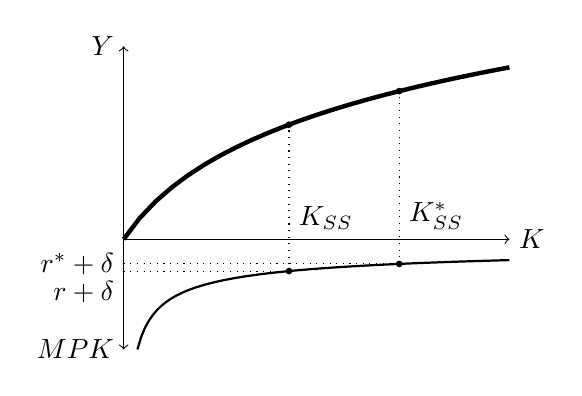
\begin{tikzpicture}[scale=.7]
        \draw [<->] (0,-2) -- (0,3.5); 
        \draw [->] (0,0) -- (7,0);
        \node [right] at (7,0) {$K$};
        \node [left] at (0,-2) {$MPK$};
        \node [left] at (0,3.5) {$Y$};  
        \draw[ultra thick, domain=0:7] plot (\x, {1.5*ln(1+\x)});
        \draw[thick,samples=100,domain=0.25:7] plot(\x, {-pow(\x, -0.5)});
        \draw [dotted] (0,-0.577) -- (3,-0.577);
        \draw [dotted] (3,-0.577) -- (3,2.079);
        \draw [fill] (3,-0.577) circle [radius=0.05];
        \draw [fill] (3,2.079) circle [radius=0.05];
        \node [below left] at (0,-0.577) {$r+\delta$};
        \node [above right] at (3,0) {$K_{SS}$};
        \draw [dotted] (0,-0.447) -- (5,-0.447);
        \draw [dotted] (5,-0.447) -- (5,2.6876);
        \draw [fill] (5,-0.447) circle [radius=0.05];
        \draw [fill] (5,2.6876) circle [radius=0.05];
        \node [left] at (0, -0.447) {$r^*+\delta$};
        \node [above right] at (5,0) {$K^*_{SS}$};
    \end{tikzpicture}
\end{figure}
\item In the language of GTAP:
\begin{center}
\textbf{Shock} \textcolor{OliveGreen}{f\_rorc}(``CHN") = -10.0
\footnote{The GTAP model is modefied: rorc(r)=rorc + f\_rorc(r).
See Gretton (2016) for more detail. \footfullcite{gretton2016}}
\end{center}
\end{itemize}
\end{frame}

\begin{frame}{Simulation Result III}{A Reduction in Required Rate of Return on Capital}
\begin{table}
\begin{threeparttable}
\def\theadset{\def\arraytretch{1.5}}
\def\arraystretch{1.2}
\small
\begin{tabular}{lcccc}
\hline\hline
    & \thead{Read GDP\\\emph{\% change}} 
    & \thead{Capital accumulation\\\emph{\% change}} 
    & \thead{Trade balance to\\income ratio} \\
\hline
CHN & 4.088 &	10.824 & 0.018 \\
AUS & 0.127 &	0.245 & -0.003 \\
USA & 0.023 &	0.056 & -0.002 \\
EU  & 0.003 &	0.022 & -0.002 \\
ROW & 0.035 &	0.046 & -0.002 \\
\hline\hline
\end{tabular}
\begin{tablenotes}[para,flushleft]
\footnotesize
\emph{Note:} Modelled as a 10\% reduction in overall required rate of 
capital in China. 
The model is solved using Gragg's method; the accuracy requirement is set to that 
at least 99\% of the variables are accurate to at least 4 figures. 
The extrapolation accuracy shows that we can be confident for 6 figure accuracy 
for most variables.\\
\emph{Source:} Author estimated.
\end{tablenotes}
\end{threeparttable}
\end{table}
\end{frame}

\subsection{Overall Impact}
\begin{frame}{Simulation Result IV}{Overall Impact}
\begin{table}
\begin{threeparttable}
% \caption{Simulation Result of Overall Impact}
% \label{tab:sim-all}
\def\theadset{\def\arraytretch{1.5}}
\def\arraystretch{1.2}
\small
\begin{tabular}{lcccc}
\hline\hline
    & \thead{Read GDP\\\emph{\% change}} 
    & \thead{Capital accumulation\\\emph{\% change}} 
    & \thead{Trade balance to\\income ratio} \\
\hline
CHN & 5.112 &	11.932 & 0.018 \\
AUS & 0.147 &	0.290  & -0.003 \\
USA & 0.020 &	0.045  & -0.002 \\
EU  & -0.008 &	-0.002 & -0.002 \\
ROW & 0.028 &	0.031  & -0.002 \\
\hline\hline
\end{tabular}
\begin{tablenotes}[para,flushleft]
\emph{Note:} Modelled as a 10\% reduction in required rate of capital, 
together with a uniform 1 point increase in value-added augmenting technology,  
a uniform 1 point increase in financial intermediate input augmenting technology, 
and a uniform 1 point increase in primary augmenting technology for capital.
% The model is solved using Gragg's method; the accuracy requirement is set 
% to that at least 99\% of the variables are accurate to at least 4 figures. 
% The extrapolation accuracy shows that we can be confident for 6 figure accuracy 
% for most variables.\\
\emph{Source:} Author estimated.
\end{tablenotes}
\end{threeparttable}
\end{table}   
\end{frame}


\subsection{Sector Performance}
\begin{frame}{Simulation Result V}{Sector Performance}
\begin{table}
\begin{threeparttable}
% \caption{Simulation Result of Sector Output in China (\% Change)}
% \label{tab:sim-sector}
\def\theadset{\def\arraytretch{2}}
\def\arraystretch{1.2}
\small
\begin{tabular}{lccccc}
\hline\hline
 & \thead{CHN} & \thead{AUS} & \thead{USA} & \thead{EU} & \thead{ROW} \\  
\hline
 Grains \& Crops 	            &2.702	&-0.011	&0.554	&0.238	&0.243 \\
 Livestock \& Fishing    	    &3.124	&0.716	&0.127	&0.205	&0.093 \\
 Mining      	                &4.188	&0.717	&0.328	&0.692	&0.502 \\
 Processed Food    	            &2.934	&-0.401	&0.018	&0.071	&0.050 \\
 Textiles    	                &5.619	&-2.558	&-0.976	&-1.175	&-1.413\\
 Light Manufacturing   	        &7.477	&-1.111	&-0.544	&-0.773	&-0.863\\
 Heavy Manufacturing   	        &7.477	&-1.903	&-0.493	&-0.359	&-0.813\\
 Construction       	        &2.734	&0.980	&0.783	&0.813	&0.760 \\
 Utilities       	            &5.841	&-0.277	&-0.062	&-0.117	&-0.185\\
 Transport \& Communication   	&5.467	&0.013	&0.040	&0.038	&0.053 \\
 Financial Services      	    &5.807	&0.182	&0.026	&0.066	&-0.003\\
 Dwellings         	            &6.307	&0.392	&0.075	&-0.006	&0.161 \\
%  Other Services 	            &3.215	&0.192	&0.040	&0.022	&0.132 \\
\hline\hline
\end{tabular}
% \begin{tablenotes}[para,flushleft]
% \emph{Note:} Modelled as a 10 percent reduction in required rate of capital, 
% together with a uniform 1 point increase in value-added augmenting technology,  
% a uniform 1 point increase in financial intermediate input augmenting technology, 
% and a uniform 1 point increase in primary augmenting technology for capital.
% The model is solved using Gragg's method; the accuracy requirement is set 
% to that at least 99\% of the variables are accurate to at least 4 figures. 
% The extrapolation accuracy shows that we can be confident for 6 figure accuracy 
% for most variables.\\
% \emph{Source:} Author estimated.
% \end{tablenotes}
\end{threeparttable}
\end{table}  
\end{frame}

\section{Conclusion}
\subsection{Simulation Summary}

\begin{frame}{Conclusion}{Simulation Summary}
\begin{itemize}
\item Remarkably increase in GDP and capital intensity 
\item More balanced development and more efficient resource allocation
\item Most countries in the world would also benefit indirectly
\end{itemize}
\end{frame}

% \subsection{Risk Concerns}
% \begin{frame}{Conclusion}{Risk Concerns}
% \begin{itemize}
% \item Financial liberalization is never without risk
% \item Risk concerns of financial liberalization in China
% \begin{itemize}
%     \item Asset bubble: capital flight?
%     \item Over investment: debt crisis?
%     \item Banking system collapse?
% \end{itemize}
% \item Financial liberalization should be undertaken with risk management \footfullcite{mckibbin1999}
% \end{itemize}    
% \end{frame}


% All of the following is optional and typically not needed. 
% \appendix
% \section<presentation>*{\appendixname}
% \subsection<presentation>*{References}

% \begin{frame}[allowframebreaks]
%   \frametitle<presentation>{References}
%   \printbibliography
% \end{frame}

\end{document}


